% SC1004 Chapter 3: Linear Systems & Gauss Elimination (0->100 ground-up)
\chapter{Linear Systems and Gaussian Elimination}
\label{ch:systems}

\begin{quote}
\emph{``Elimination is just organised subtraction.''} A system of equations is a puzzle of balances; Gaussian elimination solves it by the same moves you would use on paper --- swap, scale, subtract --- written as row operations on a matrix.
\end{quote}

\noindent\fbox{\parbox{\dimexpr\linewidth-2\fboxsep-2\fboxrule}{%
\textbf{From zero: no systems background needed.} We start with two lines in the plane, see the three things that can happen (one point, no point, a whole line), then grow to $m\times n$ and build an algorithm that handles them all.}}
\vspace{0.4em}

\section*{Learning Outcomes}
After this chapter you will be able to:
\begin{enumerate}[label=(L\arabic*)]
    \item write a linear system as $A\mathbf{x}=\mathbf{b}$ and as an augmented matrix $[A\mid\mathbf{b}]$;
    \item carry out Gaussian elimination to row-echelon and Gauss--Jordan forms;
    \item read off existence, uniqueness, and parametric solution sets;
    \item relate pivots, free variables, and rank to the geometry;
    \item factor $A=LU$ and use it to solve efficiently.
\end{enumerate}

% ============================================================
\section{Systems as Matrices}
\label{sec:systems-matrix}
A \emph{linear equation} is $a_1x_1+\cdots+a_nx_n=b$. A \emph{system} of $m$ such equations is
\[
  A\mathbf{x}=\mathbf{b},\quad A\in\mathbb{R}^{m\times n},\ \mathbf{x}\in\mathbb{R}^n,\ \mathbf{b}\in\mathbb{R}^m.
\]
The \emph{augmented matrix} $[A\mid\mathbf{b}]$ keeps all the data in one table.

\begin{figure}[h]
\centering
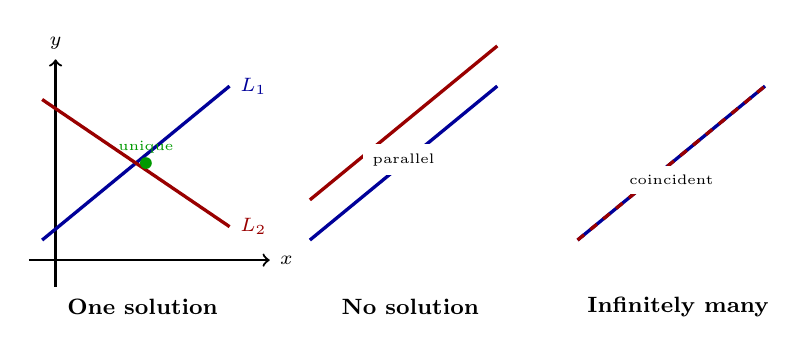
\begin{tikzpicture}[scale=0.85,every node/.style={font=\scriptsize}]
  \draw[->,thick] (-0.4,0)--(3.2,0) node[right] {$x$};
  \draw[->,thick] (0,-0.4)--(0,3.0) node[above] {$y$};
  % one intersection
  \begin{scope}
    \draw[very thick,blue!60!black] (-0.2,0.3)--(2.6,2.6) node[right] {$L_1$};
    \draw[very thick,red!60!black] (-0.2,2.4)--(2.6,0.5) node[right] {$L_2$};
    \fill[green!60!black] (1.35,1.45) circle (2.5pt) node[above,font=\tiny] {unique};
    \node[font=\footnotesize\bfseries] at (1.3,-0.7) {One solution};
  \end{scope}
  \begin{scope}[xshift=4.0cm]
    \draw[very thick,blue!60!black] (-0.2,0.3)--(2.6,2.6);
    \draw[very thick,red!60!black] (-0.2,0.9)--(2.6,3.2);
    \node[font=\tiny,fill=white] at (1.2,1.5) {parallel};
    \node[font=\footnotesize\bfseries] at (1.3,-0.7) {No solution};
  \end{scope}
  \begin{scope}[xshift=8.0cm]
    \draw[very thick,blue!60!black] (-0.2,0.3)--(2.6,2.6);
    \draw[very thick,red!60!black,dashed] (-0.2,0.3)--(2.6,2.6);
    \node[font=\tiny,fill=white] at (1.2,1.2) {coincident};
    \node[font=\footnotesize\bfseries] at (1.3,-0.7) {Infinitely many};
  \end{scope}
\end{tikzpicture}
\caption{Three geometries for two equations in two unknowns. With more variables the same trichotomy holds.}
\label{fig:three-cases}
\end{figure}

For $n>2$ we cannot draw, but algebra does not care: the same three outcomes occur.

\section{Row Operations and Echelon Form}
\label{sec:row-ops}
Elimination uses three \emph{elementary row operations} on $[A\mid\mathbf{b}]$, each reversible and preserving the solution set:
\begin{enumerate}[label=(R\arabic*)]
    \item Swap two rows: $R_i\leftrightarrow R_j$.
    \item Scale a row: $R_i\gets cR_i$, $c\neq0$.
    \item Add a multiple: $R_i\gets R_i+cR_j$, $i\neq j$.
\end{enumerate}

\begin{definition}[Row-echelon form (REF)]
A matrix is in REF if (i) all zero rows are at the bottom, (ii) each leading entry (pivot) is to the right of the one above, (iii) pivots may be any nonzero. In \emph{reduced} REF (RREF), each pivot is $1$ and is the only nonzero in its column.
\end{definition}

\begin{figure}[h]
\centering
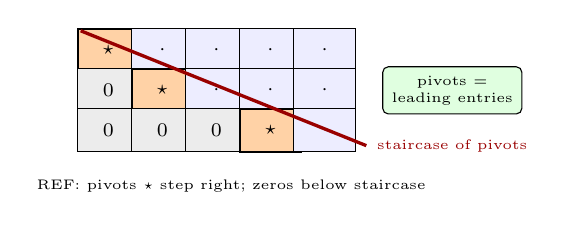
\begin{tikzpicture}[scale=0.78,every node/.style={font=\scriptsize}]
  \foreach \r in {0,...,2} \foreach \c in {0,...,4} {
    \pgfmathsetmacro{\shade}{(\r==0 && \c==0) || (\r==1 && \c==1) || (\r==2 && \c==3) ? 1 : 0}
    \ifnum\shade=1
      \node[draw,thick,minimum width=0.78cm,minimum height=0.55cm,fill=orange!35] at (\c*0.88,\r*-0.65) {$\star$};
    \else
      \pgfmathparse{(\r==0 || (\r==1 && \c>=1) || (\r==2 && \c>=3)) ? 1 : 0}
      \ifnum\pgfmathresult=1
        \node[draw,minimum width=0.78cm,minimum height=0.55cm,fill=blue!7] at (\c*0.88,\r*-0.65) {$\cdot$};
      \else
        \node[draw,minimum width=0.78cm,minimum height=0.55cm,fill=gray!15] at (\c*0.88,\r*-0.65) {$0$};
      \fi
    \fi
  }
  \draw[very thick,red!60!black] (-0.45,0.32)--(4.2,-1.55) node[right,font=\tiny] {staircase of pivots};
  \node[font=\tiny] at (2.0,-2.2) {REF: pivots $\star$ step right; zeros below staircase};
  \node[draw,rounded corners=2pt,fill=green!12,font=\tiny,align=center] at (5.6,-0.65) {pivots $=$\\leading entries};
\end{tikzpicture}
\caption{Shape of a row-echelon matrix. The staircase separates the pivot columns from free columns.}
\label{fig:echelon}
\end{figure}

\emph{Gaussian elimination:} work column by column, pick a pivot, clear below with (R3), move to next row/column. \emph{Gauss--Jordan} continues upward to clear above pivots, reaching RREF.

\begin{example}[Elimination by hand]
Solve
\[
\begin{cases}
  x+2y+z=4\\ 2x+5y+z=7\\ x+y- z=0
\end{cases}\quad
\left[\begin{array}{ccc|c}1&2&1&4\\2&5&1&7\\1&1&-1&0\end{array}\right]
\xrightarrow{R_2-2R_1,\;R_3-R_1}
\left[\begin{array}{ccc|c}1&2&1&4\\0&1&-1&-1\\0&-1&-2&-4\end{array}\right]
\xrightarrow{R_3+R_2}
\left[\begin{array}{ccc|c}1&2&1&4\\0&1&-1&-1\\0&0&-3&-5\end{array}\right].
\]
Back substitution: $z=5/3$, $y=-1+z=2/3$, $x=4-2y-z=1$. Unique solution $\mathbf{x}=[1,2/3,5/3]^T$. If a row became $[0\;0\;0\mid1]$, inconsistency --- no solution.
\end{example}

\section{Solution Sets: Pivots vs.\ Free Variables}
\label{sec:solution-sets}
Each column with a pivot is a \emph{pivot column}; the rest are \emph{free}. Free variables become parameters.

\begin{theorem}[Existence and uniqueness]
$A\mathbf{x}=\mathbf{b}$ has a solution iff $\operatorname{rank}(A)=\operatorname{rank}([A\mid\mathbf{b}])$ (no pivot in the augmented column). It is unique iff every variable column is a pivot column (no free variables).
\end{theorem}

When free variables exist, the solution is an affine subspace:
\[
  \mathbf{x}=\mathbf{p}+t_1\mathbf{v}_1+\cdots+t_k\mathbf{v}_k,
\]
$\mathbf{p}$ a particular solution, $\{\mathbf{v}_i\}$ span the homogeneous solutions $A\mathbf{x}=\mathbf{0}$ (the null space, Ch.~4).

\begin{figure}[h]
\centering
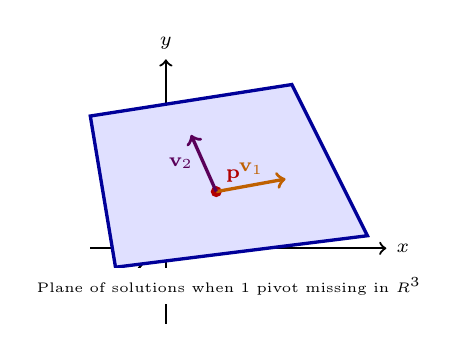
\begin{tikzpicture}[scale=0.80,every node/.style={font=\scriptsize}]
  \draw[->,thick] (-1.2,0)--(3.5,0) node[right] {$x$};
  \draw[->,thick] (0,-1.2)--(0,3.0) node[above] {$y$};
  \draw[->,thick] (-0.8,-0.8)--(1.5,2.2) node[above] {$z$};
  \fill[blue!12] (-0.8,-0.3)--(3.2,0.2)--(2.0,2.6)--(-1.2,2.1)--cycle;
  \draw[very thick,blue!60!black] (-0.8,-0.3)--(3.2,0.2)--(2.0,2.6)--(-1.2,2.1)--cycle;
  \fill[red!70!black] (0.8,0.9) circle (2.5pt) node[above right] {$\mathbf{p}$};
  \draw[->,very thick,orange!75!black] (0.8,0.9)--(1.9,1.1) node[midway,above] {$\mathbf{v}_1$};
  \draw[->,very thick,violet!70!black] (0.8,0.9)--(0.4,1.8) node[midway,left] {$\mathbf{v}_2$};
  \node[font=\tiny,fill=white] at (1.0,-0.6) {Plane of solutions when 1 pivot missing in $\mathbb{R}^3$};
\end{tikzpicture}
\caption{With free variables, solutions form $\mathbf{p}+\operatorname{span}\{\mathbf{v}_i\}$ --- a point, line, plane, or hyperplane.}
\label{fig:solution-affine}
\end{figure}

\section{LU Factorisation}
\label{sec:lu}
Elimination records its multipliers in $L$ (unit lower-triangular) so that $A=LU$ with $U$ the REF. Then $A\mathbf{x}=\mathbf{b}$ becomes $L\mathbf{y}=\mathbf{b}$ (forward substitution) then $U\mathbf{x}=\mathbf{y}$ (back substitution) --- $O(n^2)$ per new $\mathbf{b}$ after one $O(n^3)$ factorisation. With row swaps, $PA=LU$.

\begin{example}[Python --- elimination and LU]
\begin{lstlisting}[language=Python]
import numpy as np
from scipy.linalg import lu
A = np.array([[1.,2.,1.],[2.,5.,1.],[1.,1.,-1.]])
b = np.array([4.,7.,0.])
x = np.linalg.solve(A, b)
print(x)  # [1. 0.666... 1.666...]
P, L, U = lu(A)
print(np.allclose(P@L@U, A))  # True
\end{lstlisting}
If \texttt{np.linalg.matrix\_rank(A)} $<n$, expect either no or infinitely many solutions --- check augmented rank.
\end{example}

% ============================================================

% --- Additional depth: Rank, nullity preview, and iterative view ---
\section{Rank and Its Geometry}
\label{sec:rank-geom}
The number of pivots $r=\operatorname{rank}(A)$ counts independent equations (or independent columns). Full row rank ($r=m$) means $A\mathbf{x}=\mathbf{b}$ solvable for every $\mathbf{b}$; full column rank ($r=n$) means at most one solution for each $\mathbf{b}$. When $r<\min(m,n)$, both existence and uniqueness can fail depending on $\mathbf{b}$.

\begin{theorem}[Rank of products and sums]
$\operatorname{rank}(AB)\le\min(\operatorname{rank}A,\operatorname{rank}B)$; $\operatorname{rank}(A+B)\le\operatorname{rank}A+\operatorname{rank}B$. Row operations preserve rank (they are left-multiplication by invertible $E$).
\end{theorem}

\section{Computational Cost and Pivoting}
\label{sec:pivot-cost}
Elimination on $n\times n$ costs $\sim\frac23n^3$ flops (floating-point ops); forward/back substitution $O(n^2)$. Partial pivoting (swap to bring largest $|a_{ik}|$ to pivot) avoids division by tiny numbers and controls error growth (factor $\le2^{n-1}$ worst-case, tiny in practice). Complete pivoting (row+column swaps) is more stable but costlier. Libraries (LAPACK) use blocked $LU$ for cache efficiency.

\begin{example}[When pivoting matters]
$A=\begin{bmatrix}10^{-12}&1\\1&1\end{bmatrix}$ without pivoting: first pivot $10^{-12}$ causes catastrophic cancellation in $R_2\gets R_2-10^{12}R_1$. Swapping rows first gives pivot $1$, stable elimination.
\end{example}



\begin{remark}[Geometric reading of REF]
Each pivot column corresponds to a direction that is constrained; each free column is a degree of freedom. So $\operatorname{rank}A$ is the dimension of the column space (how many independent constraints), and $n-\operatorname{rank}A$ is the dimension of the solution line/plane when $\mathbf{b}$ is consistent. This foreshadows Ch.~5's rank--nullity.
\end{remark}

\begin{example}[No solution vs.\ infinitely many]
$A=\begin{bmatrix}1&1\\2&2\end{bmatrix}$, $\mathbf{b}_1=[1,3]^T$: augmented REF $\begin{bmatrix}1&1&1\\0&0&1\end{bmatrix}$ --- pivot in augmented column, no solution (parallel lines). $\mathbf{b}_2=[1,2]^T$: $\begin{bmatrix}1&1&1\\0&0&0\end{bmatrix}$ --- free $x_2=t$, solutions $[1-t,t]^T$ (coincident lines).
\end{example}


\section{Chapter Notes}
Gauss described elimination circa 1809 (least squares); Jordan pushed to RREF. $LU$ is how libraries actually solve $A\mathbf{x}=\mathbf{b}$; QR (Ch.~6) is the stable alternative for least squares. Pivoting (partial: largest in column) controls round-off.

% ============================================================
\section{Exercises}
\label{sec:ch03-exercises}
\begin{enumerate}[label=E3.\arabic*, leftmargin=*, itemsep=0.8em]
\item \textbf{REF by hand.} Reduce $\begin{bmatrix}1&2&3&9\\2&4&5&13\\1&0&-1&-1\end{bmatrix}$ to REF and RREF. Identify pivots and free variables; write all solutions.
\item \textbf{Trichotomy.} Give matrices $A$ and vectors $\mathbf{b}_1,\mathbf{b}_2,\mathbf{b}_3$ ($2\times2$) exhibiting the three cases: unique solution, no solution, infinitely many. Explain via ranks of $A$ and $[A\mid\mathbf{b}]$.
\item \textbf{Homogeneous.} Show the solution set of $A\mathbf{x}=\mathbf{0}$ is closed under addition and scaling. Find a basis for it when $A=\begin{bmatrix}1&2&-1&0\\0&1&1&1\end{bmatrix}$.
\item \textbf{LU.} Compute $L$ and $U$ (no pivoting) for $A=\begin{bmatrix}2&1&1\\4&5&2\\2&1&-1\end{bmatrix}$ by recording multipliers. Verify $A=LU$ and solve $A\mathbf{x}=[1,2,0]^T$ via $L,U$.
\item \textbf{Coding.} Write \texttt{rref(A)} (Gauss--Jordan, partial pivoting, tolerance $10^{-10}$) returning RREF and pivot columns. Test on random $3\times5$ matrices and compare pivot columns with \texttt{np.linalg.matrix\_rank}.
\end{enumerate}
% End of Chapter 3
